\documentclass{article}
\usepackage{listings}
\usepackage{xcolor}
\usepackage{graphicx} % Required for inserting images
\usepackage{tikz} % Drawing
\usepackage[backend=biber,style=apa]{biblatex}
\usepackage{amsmath}
\usepackage{algorithm}
\usepackage{algorithmic}
\usepackage{booktabs}
\usepackage{multirow}

\lstset{ 
  language=R,
  backgroundcolor=\color{white},   
  basicstyle=\footnotesize\ttfamily,    
  breaklines=true,                    
  captionpos=b,                     
  keepspaces=true,                   
  numbers=left,                     
  numberstyle=\tiny\color{gray},  
  stringstyle=\color{purple},     
  commentstyle=\color{gray},  
  keywordstyle=\color{blue},  
  showstringspaces=false
}

% load bib
\addbibresource{reference.bib}

\title{BKT: A Bayesian Knowledge Tracing Package for the R Environment}
\author{Yuhao Yuan, Biying Zhou, Feng Ji}
\date{\today}

\begin{document}

\maketitle

% some notes
\begin{itemize}
    \item Target Journal: Journal of Statistical Software, Behavior Research Methods, Or Applied Psychological Measurement
    \item \textbf{Storyline} Introduce BKT and its variant, showcase its usefulness in an empirical data and/or a simulated data $\rightarrow$ give a simple tutorial involving how to use it in R.
\end{itemize}
\section{Introduction}

Bayesian Knowledge Tracing (BKT) is a widely used model for understanding student learning over time, particularly in educational technology applications (\cite{corbett1994knowledge}). Over the years, several variants of the BKT model have been proposed to enhance its predictive capabilities and flexibility. 

BKT has evolved into various models, each addressing different aspects of student learning and behavior. The Prior Per Student (PPS) Model (\cite{multiprior}) builds upon BKT by individualizing the prior rate for each student, diverging from the traditional BKT assumption of a shared global prior rate. The Item Order Effect (IOE) Model (\cite{multipair}) extends BKT by localizing the learning rate to each pair of items, allowing for a more nuanced representation of learning progression across different items. The Item Difficulty Effect (IDE) Model (\cite{multiguess}) enhances BKT by personalizing the guess and slip rates for each item, instead of assuming a uniform global rate. Lastly, the Learning and Forgetting Behavior (LFB) Model (\cite{forget}) introduces the concept of forgetting into the learning process, acknowledging that forgetting is an integral part of how students retain and lose knowledge over time.

However, despite the availability of multiple BKT variants, only one fully implemented software package, pyBKT, exists for Python (\cite{badrinath2021pybkt}). This package serves as the primary tool for applying BKT models in the Python environment. In addition to pyBKT, there is also the standard-BKT command-line tool implemented in C++ (\cite{standardBKT}). This tool focuses on parameter estimation for basic BKT models.

To extend the accessibility and functionality of BKT, this R package has been developed, replicating the core features of pyBKT and making them available for R users. With this implementation, users can now seamlessly apply Bayesian Knowledge Tracing models in R, thus broadening the accessibility of this important educational tool.

\section{Model description}

\subsection{Bayesian Knowledge Tracing}
Bayesian Knowledge Tracing is a probabilistic model designed to track a learner’s state of knowledge over time, specifically focusing on transitions between "unknown" and "known" states for a particular skill or concept. BKT assumes that a learner has a probability of transitioning from an unknown state to a known state based on the correctness of their responses during learning activities. Here, we provide detailed explanations of the learning process as abstracted by the BKT model.

In general, people acquire knowledge by engaging in learning activities. Learner's knowledge state can be observed by changes in their performance in these activities. This learning process is illustrated in Figure 1.

\begin{center}
    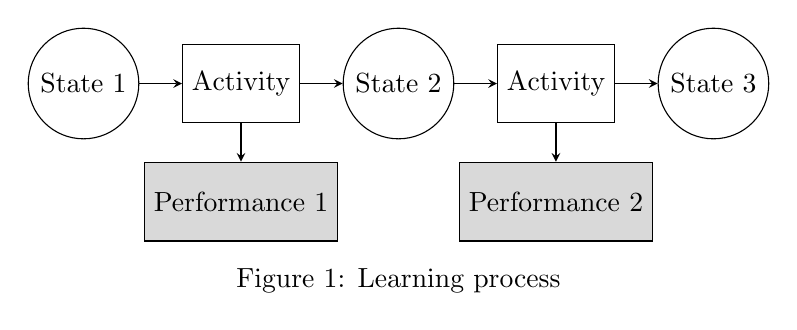
\begin{tikzpicture}
        % Define styles
        \tikzset{
            state/.style={circle, draw, minimum size=1cm},
            activity/.style={rectangle, draw, minimum size=1cm},
            performance/.style={rectangle, draw, fill=gray!30, minimum size=1cm},
            arrow/.style={->,>=stealth}
        }
        
        % Nodes
        \node[state] (state_node_1) at (0,0) {State 1};
        \node[activity] (activity_node_1) at (2,0) {Activity};
        \node[performance] (performance_node_1) at (2,-1.5) {Performance 1};
        \node[state] (state_node_2) at (4,0) {State 2};
        
        \node[activity] (activity_node_2) at (6,0) {Activity};
        \node[performance] (performance_node_2) at (6,-1.5) {Performance 2};
        \node[state] (state_node_3) at (8,0) {State 3};
        
        % Arrows
        \draw[arrow] (state_node_1) -- (activity_node_1);
        \draw[arrow] (activity_node_1) -- (state_node_2);
        \draw[arrow] (activity_node_1) -- (performance_node_1);
        \draw[arrow] (state_node_2) -- (activity_node_2);
        \draw[arrow] (activity_node_2) -- (state_node_3);
        \draw[arrow] (activity_node_2) -- (performance_node_2);
    
        % Footnote
        \node at (4,-2.5) {Figure 1: Learning process};
    \end{tikzpicture}
\end{center}

Another assumption of the BKT model is the binary nature of learning states and the impact of activities on these states. BKT assumes that a learner is either in a known state or an unknown state. By participating in an activity, a learner in the unknown state has a chance to transition to the known state. Therefore, learning activities cause three types of state changes: remaining known, learning (transitioning from unknown to known), and remaining unknown. This is illustrated in Figure 2. Note that the transition from the unknown state to the known state represents the learning process as a hidden Markov model in the BKT framework.

\begin{center}
    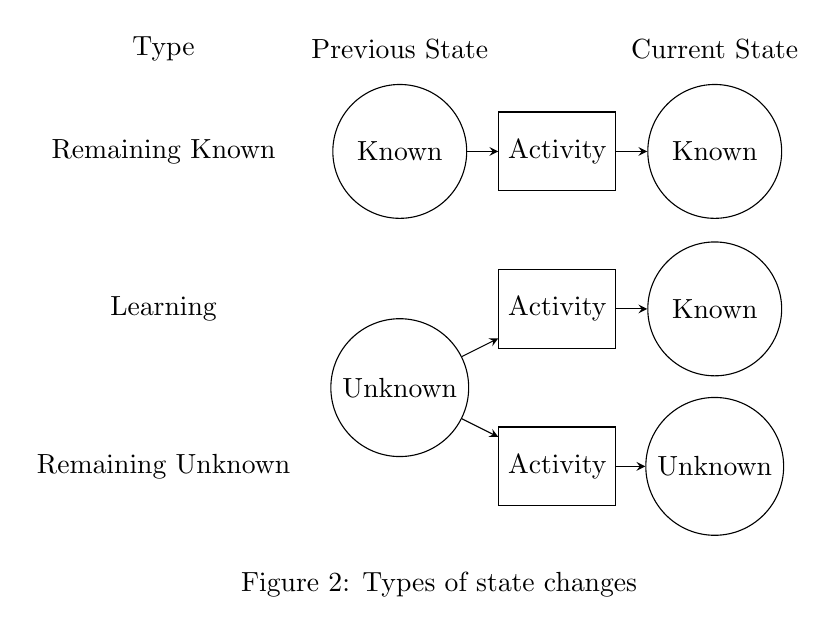
\begin{tikzpicture}
        % Define styles
        \tikzset{
            state/.style={circle, draw, minimum size=1.7cm},
            activity/.style={rectangle, draw, minimum size=1cm},
            arrow/.style={->,>=stealth}
        }
        
        % Nodes
        \node[] () at (-3,1.3) {Type};
        \node[] () at (0,1.3) {Previous State};
        \node[] () at (4,1.3) {Current State};

        \node[] () at (-3,0) {Remaining Known};
        \node[state] (state_node_1) at (0,0) {Known};
        \node[activity] (activity_node_1) at (2,0) {Activity};
        \node[state] (state_node_2) at (4,0) {Known};
        
        \node[] () at (-3,-2) {Learning};
        \node[state] (state_node_3) at (0,-3) {Unknown};
        \node[activity] (activity_node_2) at (2,-2) {Activity};
        \node[state] (state_node_4) at (4,-2) {Known};
        
        \node[] () at (-3,-4) {Remaining Unknown};
        % \node[state] (state_node_5) at (0,-4) {Unknown};
        \node[activity] (activity_node_3) at (2,-4) {Activity};
        \node[state] (state_node_6) at (4,-4) {Unknown};
        
        % Arrows
        \draw[arrow] (state_node_1) -- (activity_node_1);
        \draw[arrow] (activity_node_1) -- (state_node_2);
        \draw[arrow] (state_node_3) -- (activity_node_2);
        \draw[arrow] (activity_node_2) -- (state_node_4);
        \draw[arrow] (state_node_3) -- (activity_node_3);
        \draw[arrow] (activity_node_3) -- (state_node_6);
    
        % Footnote
        \node at (0.5,-5.5) {Figure 2: Types of state changes};
    \end{tikzpicture}
\end{center}

One can infer a learner’s knowledge state by observing their performance on activities. However, there are two common scenarios to consider: a learner in an unknown state answering correctly (guessing) and a learner in a known state answering incorrectly (slipping). The relationship between activity performance and knowledge state is shown in Figure 3.

\begin{center}
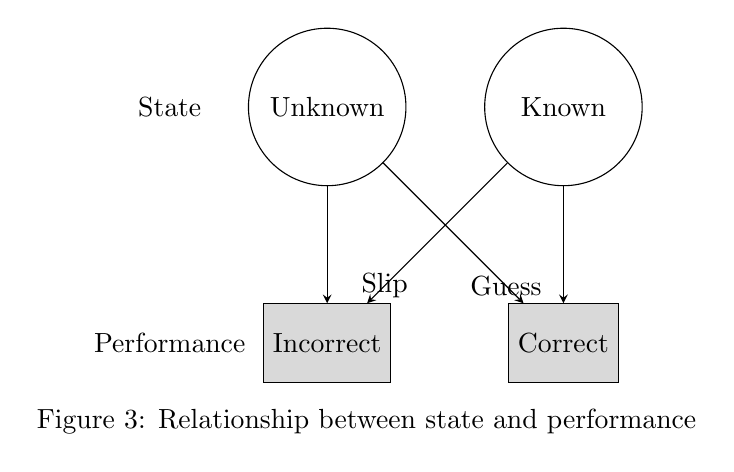
\begin{tikzpicture}
    % Define styles
    \tikzset{
        state/.style={circle, draw, minimum size=2cm},
        performance/.style={rectangle, draw, fill=gray!30, minimum size=1cm},
        arrow/.style={->,>=stealth}
    }
    
    % Nodes
    \node[] (state_label) at (-1,0) {State};
    \node[] (performance_label) at (-1,-3) {Performance};
    \node[state] (not_known) at (1,0) {Unknown};
    \node[state] (known) at (4,0) {Known};
    \node[performance] (incorrect) at (1,-3) {Incorrect};
    \node[performance] (correct) at (4,-3) {Correct};
    
    % Arrows
    \draw[arrow] (not_known) -- (incorrect);
    \draw[arrow] (not_known) -- (correct) node[very near end] {Guess};
    \draw[arrow] (known) -- (correct);
    \draw[arrow] (known) -- (incorrect) node[very near end] {Slip};

    % Footnote
    \node at (1.5,-4) {Figure 3: Relationship between state and performance};
\end{tikzpicture}
\end{center}

BKT provides a static approach, using specific and quantified probability descriptions to calculate the likelihood of the learning process.

In BKT terminology, we define the following:

1. \textbf{Answer}  
The answer for an activity, denoted as \( a \), represents the response given by a learner during the activity. According to BKT assumptions, its value is binary, either 0 or 1.

The variable \textbf{Answer} is the only input variable in this model.

2. \textbf{Prior}  
The prior rate, \( P_p \), represents the probability that a learner is initially in the known state.

3. \textbf{Learn}  
The learning rate, \( P_l \), indicates the probability that a learner transitions to the known state through learning.

4. \textbf{Slip}  
The slip rate, \( P_s \), denotes the probability that a learner in the known state answers incorrectly.

5. \textbf{Guess}  
The guess rate, \( P_g \), represents the probability that a learner in the unknown state answers correctly.

These four variables (\textbf{Prior} \textbf{Learn} \textbf{Slip} \textbf{Guess}) are global parameters that remain constant throughout the model.

6. \textbf{Know}  
The known rate, \( \theta \), reflects the probability that a learner is in the known state. Unlike the other parameters, \textbf{Know} is dynamic and updates iteratively as the model progresses.

For a learning process with an answer vector \( (a_1, a_2, \dots, a_i, \dots, a_S) \), where $S$ is the total number of items and the likelihood of the sequence in the BKT model is calculated as follows:

For each answer \( a_i \), let \(\theta_{i}\) denote the known rate before the \(i\)-th activity, and \(\theta_{i+1}\) the known rate after the \(i\)-th activity. Note \(\theta_1 = P_p\). The iteration of \(\theta_{i+1}\) is as follows:

First, calculate \(\theta'\), the updated known rate using Bayes' rule based on the observed answer \( a_i \):
\[
\theta' = 
\begin{cases} 
    \frac{\theta_{i} P_s}{\theta_{i} P_s + (1 - \theta_{i}) (1 - P_g)}, & \text{if } a_i = 0 \\[10pt]
    \frac{\theta_{i} (1 - P_s)}{\theta_{i} (1 - P_s) + (1 - \theta_{i}) P_g}, & \text{if } a_i = 1 
\end{cases}
\]

Figure 4 illustrates the Bayes update process.

\begin{center}
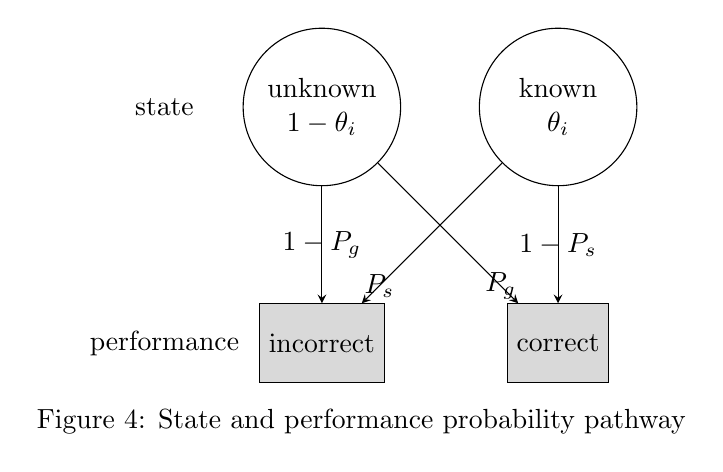
\begin{tikzpicture}
    % Define styles
    \tikzset{
        state/.style={circle, draw, minimum size=2cm},
        performance/.style={rectangle, draw, fill=gray!30, minimum size=1cm},
        arrow/.style={->,>=stealth}
    }
    
    % Nodes
    \node[] (state_node) at (-1,0) {state};
    \node[] (performance_node) at (-1,-3) {performance};
    \node[state] (not_known) at (1,0) {\parbox{1.5cm}{\centering unknown \\ \(1 - \theta_i\)}};
    \node[state] (known) at (4,0) {\parbox{1.5cm}{\centering known \\ \(\theta_{i}\)}};
    \node[performance] (incorrect) at (1,-3) {incorrect};
    \node[performance] (correct) at (4,-3) {correct};
    
    % Arrows
    \draw[arrow] (not_known) -- (incorrect) node[midway] {$1 - P_g$};
    \draw[arrow] (not_known) -- (correct) node[very near end] {$P_g$};
    \draw[arrow] (known) -- (correct) node[midway] {$1 - P_s$};
    \draw[arrow] (known) -- (incorrect) node[very near end] {$P_s$};

    % Figure label
    \node at (1.5,-4) {Figure 4: State and performance probability pathway};
\end{tikzpicture}
\end{center}

Then, update \(\theta_{i+1}\) by incorporating the potential learning effect based on \(\theta'\).

\[
\theta_{i+1} = \theta' + (1 - \theta') P_l    
\]

Now we know all learn rate before each activity \(\theta_i\), we use them to calculate the probability of each activity outcome.

\[
    Lik_i = 
    \begin{cases} 
        P_s \theta_{i} + (1 - P_g) (1 - \theta_i), & \text{if } a_i = 0 \\[10pt]
        (1 - P_s) \theta_{i} + P_g (1 - \theta_i), & \text{if } a_i = 1 
    \end{cases}
\]

So the total learn process's probability is

\[
    Lik = \prod Lik_i
\]

We can utilize the standard expectation-maximization (EM) algorithm to determine the global parameters (\(P_p, P_l, P_s, P_g\)). The EM algorithm is particularly well-suited for this task because the knowledge state of the learner is a latent variable—an unobservable factor that influences the observed performance. Directly maximizing $Lik$ is challenging due to the need to sum over all possible latent states. The EM algorithm simplifies this by iteratively estimating the expected contribution of latent states (E-step) and optimizing the parameters given these estimates (M-step), ensuring a systematic and efficient approach to converge to the optimal parameter estimates. The detailed computational steps of the EM algorithm are provided in Section Estimation.

The basic Bayesian Knowledge Tracing (BKT) model is involved here. However, it should be noted that the basic BKT model has certain limitations. The most significant issue is that it presupposes a large number of global parameters. As a result of applying these global parameters to local scenarios, numerous variants of the BKT model have emerged. At the same time, by expanding the functionality of the BKT model, some variant BKT models have also been proposed.

\subsection{BKT Variants}

% variant              name                                                        url              
% forget               Knowledge Tracing and Forgets Models                https://dl.acm.org/doi/abs/10.1145/3511808.3557622
% multilearn         Item Learning Effect Model                            http://ml4ed.cc/attachments/XuY.pdf
% multiguess        Item Difficulty Effect Mode                            https://link.springer.com/chapter/10.1007/978-3-642-22362-4_21
% multiprior          Prior per Student Model                              https://link.springer.com/chapter/10.1007/978-3-642-13470-8_24
% multipair           Item Order Effect Model                              https://eric.ed.gov/?id=ED539081
% fixed
Before introducing variants, we need to know how the basic BKT handles learning processes of multiple students.

In general, BKT calculate each student learning process likelihood individually while using same global parameters as shown in Figure 5.

\begin{center}
    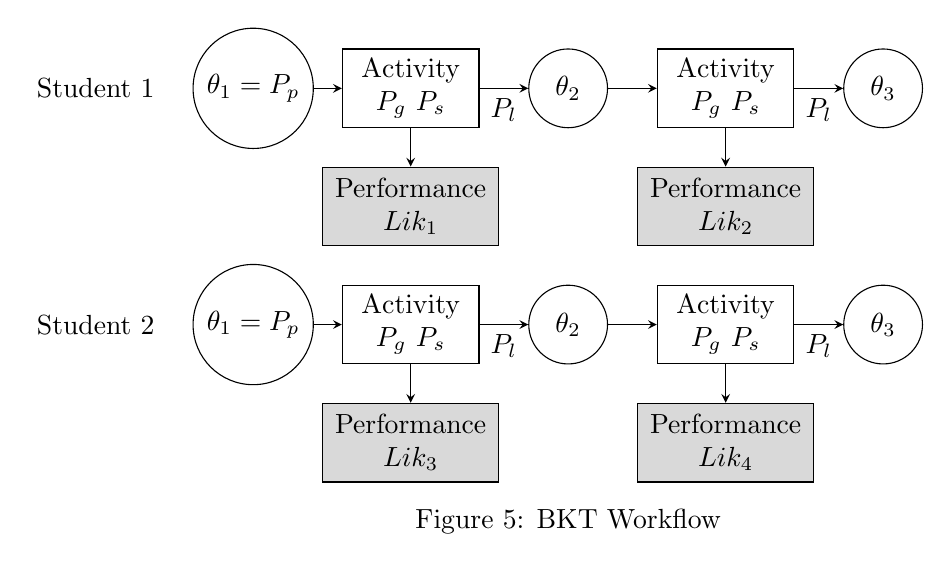
\begin{tikzpicture}
        % Define styles
        \tikzset{
            state/.style={circle, draw, minimum size=1cm},
            activity/.style={rectangle, draw, minimum size=1cm},
            performance/.style={rectangle, draw, fill=gray!30, minimum size=1cm},
            arrow/.style={->,>=stealth}
        }
        
        % Nodes
        \node[] () at (-2,0) {Student 1};
        \node[state] (state_node_1) at (0,0) {$\theta_1 = P_p$};
        \node[activity] (activity_node_1) at (2,0) {\parbox{1.5cm}{\centering Activity \\ $P_g \ P_s$}};
        \node[performance] (performance_node_1) at (2,-1.5) {\parbox{2cm}{\centering Performance \\ $Lik_1$}};
        \node[state] (state_node_2) at (4,0) {$\theta_2$};
        
        \node[activity] (activity_node_2) at (6,0) {\parbox{1.5cm}{\centering Activity \\ $P_g \ P_s$}};
        \node[performance] (performance_node_2) at (6,-1.5) {\parbox{2cm}{\centering Performance \\ $Lik_2$}};
        \node[state] (state_node_3) at (8,0) {$\theta_3$};
        
        % Arrows
        \draw[arrow] (state_node_1) -- (activity_node_1);
        \draw[arrow] (activity_node_1) -- (state_node_2) node[midway, below] {$P_l$};
        \draw[arrow] (activity_node_1) -- (performance_node_1);
        \draw[arrow] (state_node_2) -- (activity_node_2);
        \draw[arrow] (activity_node_2) -- (state_node_3) node[midway, below] {$P_l$};
        \draw[arrow] (activity_node_2) -- (performance_node_2);
    

        % student 2
        \node[] () at (-2,-3) {Student 2};
        \node[state] (state_node_2) at (0,-3) {$\theta_1 = P_p$};
        \node[activity] (activity_node_2) at (2,-3) {\parbox{1.5cm}{\centering Activity \\ $P_g \ P_s$}};
        \node[performance] (performance_node_2) at (2,-4.5) {\parbox{2cm}{\centering Performance \\ $Lik_3$}};
        \node[state] (state_node_3) at (4,-3) {$\theta_2$};
        \node[activity] (activity_node_3) at (6,-3) {\parbox{1.5cm}{\centering Activity \\ $P_g \ P_s$}};
        \node[performance] (performance_node_3) at (6,-4.5) {\parbox{2cm}{\centering Performance \\ $Lik_4$}};
        \node[state] (state_node_4) at (8,-3) {$\theta_3$};
        \draw[arrow] (state_node_2) -- (activity_node_2);
        \draw[arrow] (activity_node_2) -- (state_node_3) node[midway, below] {$P_l$};
        \draw[arrow] (activity_node_2) -- (performance_node_2);
        \draw[arrow] (state_node_3) -- (activity_node_3);
        \draw[arrow] (activity_node_3) -- (state_node_4) node[midway, below] {$P_l$};
        \draw[arrow] (activity_node_3) -- (performance_node_3);

        % Footnote
        \node at (4,-5.5) {Figure 5: BKT Workflow};
    \end{tikzpicture}
\end{center}

\subsubsection{Multiple Prior}
The Prior Per Student (PPS) Model (\cite{multiprior}) is based on BKT that focuses on individualizing the prior. The BKT assumes all student share same prior rate, the global parameter \( P_p \). The PPS localizes prior rate into each student.

The main difference in the model description lies in the initial known rate.

For each student \( j \), let \( P_{p_j} \) denote their individual prior rate. Let \(\theta_{i_j}\) denote the known rate before the \(i\)-th activity of student \(j\).
Note \(\theta_{1_j} = P_{p_j} \).

The workflow of PPS is illustrated in Figure 6. Note different student uses different initial known rate \(\theta_1\).

\begin{center}
    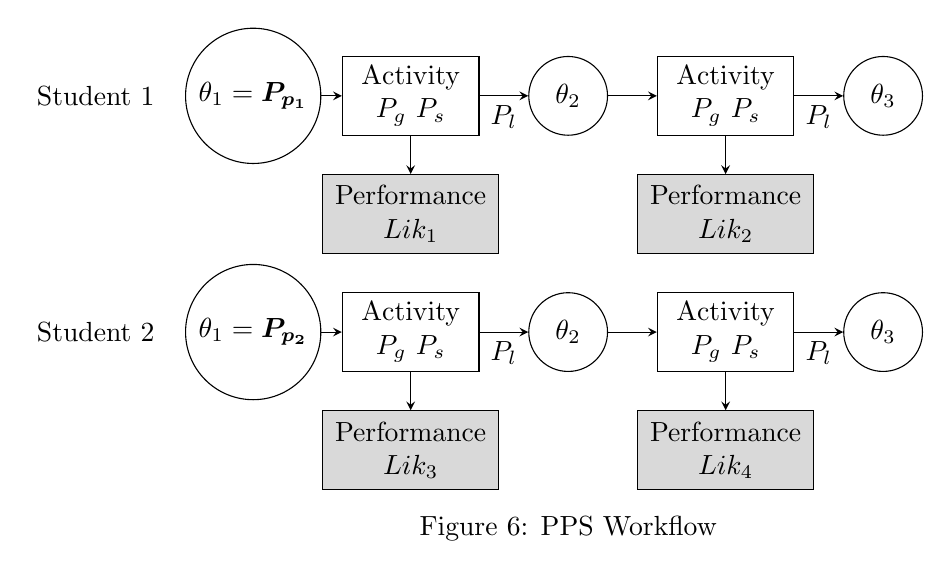
\begin{tikzpicture}
        % Define styles
        \tikzset{
            state/.style={circle, draw, minimum size=1cm},
            activity/.style={rectangle, draw, minimum size=1cm},
            performance/.style={rectangle, draw, fill=gray!30, minimum size=1cm},
            arrow/.style={->,>=stealth}
        }
        
        % Nodes
        \node[] () at (-2,0) {Student 1};
        \node[state] (state_node_1) at (0,0) {$\theta_1 = \boldsymbol{P_{p_1}}$};
        \node[activity] (activity_node_1) at (2,0) {\parbox{1.5cm}{\centering Activity \\ $P_g \ P_s$}};
        \node[performance] (performance_node_1) at (2,-1.5) {\parbox{2cm}{\centering Performance \\ $Lik_1$}};
        \node[state] (state_node_2) at (4,0) {$\theta_2$};
        
        \node[activity] (activity_node_2) at (6,0) {\parbox{1.5cm}{\centering Activity \\ $P_g \ P_s$}};
        \node[performance] (performance_node_2) at (6,-1.5) {\parbox{2cm}{\centering Performance \\ $Lik_2$}};
        \node[state] (state_node_3) at (8,0) {$\theta_3$};
        
        % Arrows
        \draw[arrow] (state_node_1) -- (activity_node_1);
        \draw[arrow] (activity_node_1) -- (state_node_2) node[midway, below] {$P_l$};
        \draw[arrow] (activity_node_1) -- (performance_node_1);
        \draw[arrow] (state_node_2) -- (activity_node_2);
        \draw[arrow] (activity_node_2) -- (state_node_3) node[midway, below] {$P_l$};
        \draw[arrow] (activity_node_2) -- (performance_node_2);
    

        % student 2
        \node[] () at (-2,-3) {Student 2};
        \node[state] (state_node_2) at (0,-3) {$\theta_1 = \boldsymbol{P_{p_2}}$};
        \node[activity] (activity_node_2) at (2,-3) {\parbox{1.5cm}{\centering Activity \\ $P_g \ P_s$}};
        \node[performance] (performance_node_2) at (2,-4.5) {\parbox{2cm}{\centering Performance \\ $Lik_3$}};
        \node[state] (state_node_3) at (4,-3) {$\theta_2$};
        \node[activity] (activity_node_3) at (6,-3) {\parbox{1.5cm}{\centering Activity \\ $P_g \ P_s$}};
        \node[performance] (performance_node_3) at (6,-4.5) {\parbox{2cm}{\centering Performance \\ $Lik_4$}};
        \node[state] (state_node_4) at (8,-3) {$\theta_3$};
        \draw[arrow] (state_node_2) -- (activity_node_2);
        \draw[arrow] (activity_node_2) -- (state_node_3) node[midway, below] {$P_l$};
        \draw[arrow] (activity_node_2) -- (performance_node_2);
        \draw[arrow] (state_node_3) -- (activity_node_3);
        \draw[arrow] (activity_node_3) -- (state_node_4) node[midway, below] {$P_l$};
        \draw[arrow] (activity_node_3) -- (performance_node_3);

        % Footnote
        \node at (4,-5.5) {Figure 6: PPS Workflow};
    \end{tikzpicture}
\end{center}

\subsubsection{Multiple Learn}

The Item Learning Effect (ILE) Model (\cite{multilearn}) is based on BKT that focuses on individualizing the learning rate. The BKT assumes all item (activity) share same learning rate, the global parameter \( P_l \). The ILE localizes learning rate into each item.

The main difference in the model description lies in the learning rate.

For each activity \( j \), let \( P_{l_j} \) denotes the learning rate.

The workflow of ILE is illustrated in Figure 7. Note there are three different activities, 1, 2 and 3.

\begin{center}
    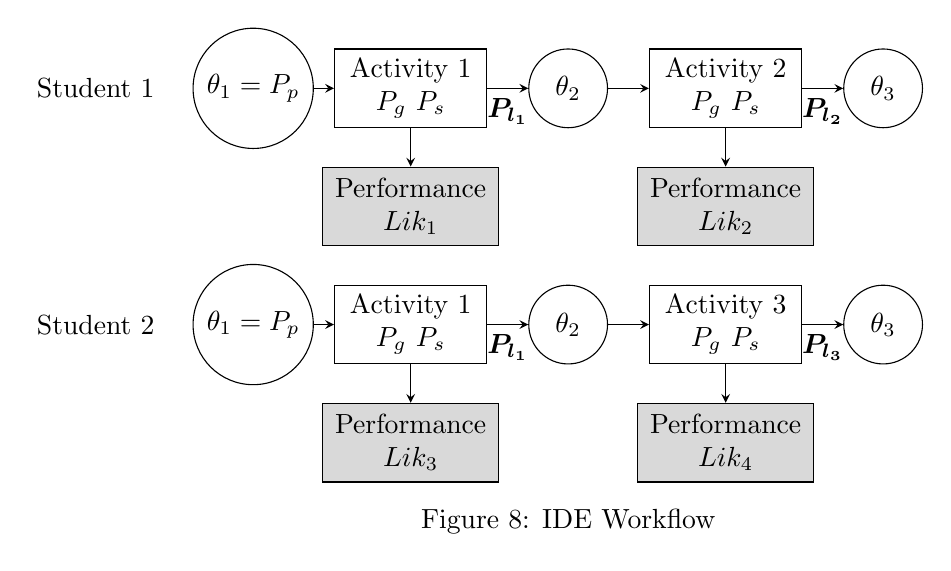
\begin{tikzpicture}
        % Define styles
        \tikzset{
            state/.style={circle, draw, minimum size=1cm},
            activity/.style={rectangle, draw, minimum size=1cm},
            performance/.style={rectangle, draw, fill=gray!30, minimum size=1cm},
            arrow/.style={->,>=stealth}
        }
        
        % Nodes
        \node[] () at (-2,0) {Student 1};
        \node[state] (state_node_1) at (0,0) {$\theta_1 = P_p$};
        \node[activity] (activity_node_1) at (2,0) {\parbox{1.7cm}{\centering Activity 1 \\ ${P_{g} \ P_{s}}$}};
        \node[performance] (performance_node_1) at (2,-1.5) {\parbox{2cm}{\centering Performance \\ $Lik_1$}};
        \node[state] (state_node_2) at (4,0) {$\theta_2$};
        
        \node[activity] (activity_node_2) at (6,0) {\parbox{1.7cm}{\centering Activity 2 \\ ${P_{g} \ P_{s}}$}};
        \node[performance] (performance_node_2) at (6,-1.5) {\parbox{2cm}{\centering Performance \\ $Lik_2$}};
        \node[state] (state_node_3) at (8,0) {$\theta_3$};
        
        % Arrows
        \draw[arrow] (state_node_1) -- (activity_node_1);
        \draw[arrow] (activity_node_1) -- (state_node_2) node[midway, below] {$\boldsymbol{P_{l_1}}$};
        \draw[arrow] (activity_node_1) -- (performance_node_1);
        \draw[arrow] (state_node_2) -- (activity_node_2);
        \draw[arrow] (activity_node_2) -- (state_node_3) node[midway, below] {$\boldsymbol{P_{l_2}}$};
        \draw[arrow] (activity_node_2) -- (performance_node_2);
    

        % student 2
        \node[] () at (-2,-3) {Student 2};
        \node[state] (state_node_2) at (0,-3) {$\theta_1 = P_p$};
        \node[activity] (activity_node_2) at (2,-3) {\parbox{1.7cm}{\centering Activity 1 \\ ${P_{g} \ P_{s}}$}};
        \node[performance] (performance_node_2) at (2,-4.5) {\parbox{2cm}{\centering Performance \\ $Lik_3$}};
        \node[state] (state_node_3) at (4,-3) {$\theta_2$};
        \node[activity] (activity_node_3) at (6,-3) {\parbox{1.7cm}{\centering Activity 3 \\ ${P_{g} \ P_{s}}$}};
        \node[performance] (performance_node_3) at (6,-4.5) {\parbox{2cm}{\centering Performance \\ $Lik_4$}};
        \node[state] (state_node_4) at (8,-3) {$\theta_3$};
        \draw[arrow] (state_node_2) -- (activity_node_2);
        \draw[arrow] (activity_node_2) -- (state_node_3) node[midway, below] {$\boldsymbol{P_{l_1}}$};
        \draw[arrow] (activity_node_2) -- (performance_node_2);
        \draw[arrow] (state_node_3) -- (activity_node_3);
        \draw[arrow] (activity_node_3) -- (state_node_4) node[midway, below] {$\boldsymbol{P_{l_3}}$};
        \draw[arrow] (activity_node_3) -- (performance_node_3);

        % Footnote
        \node at (4,-5.5) {Figure 8: IDE Workflow};
    \end{tikzpicture}
\end{center}


\subsubsection{Multiple Pair}

The Item Order Effect (IOE) Model (\cite{multipair}) is based on BKT that focuses on individualizing the learning rate. The BKT assumes all item (activity) share same learning rate, the global parameter \( P_l \). The IOE localizes learning rate into each item pairs.

The main difference in the model description lies in the learning rate.

For each activity \( i \) and activity \( j \), let \( P_{l_{ij}} \) denotes the learning rate from activity \( i \) to activity \( j \). Note \( P_{l_{0j}} \) refers initial activity learn rate.

The workflow of ILE is illustrated in Figure 9. Note there are three different activities, 1, 2 and 3 with most 6 pairs.

\begin{center}
    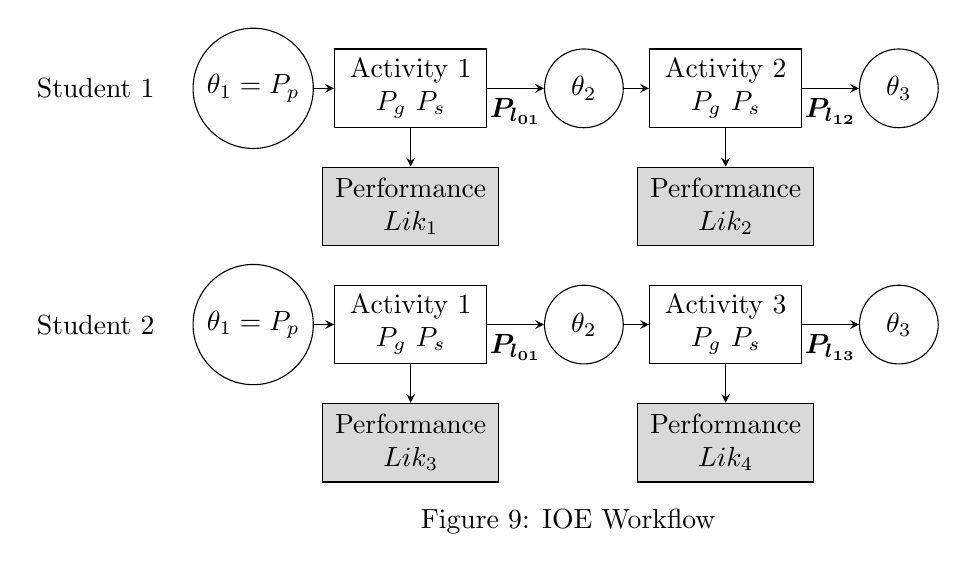
\begin{tikzpicture}
        % Define styles
        \tikzset{
            state/.style={circle, draw, minimum size=1cm},
            activity/.style={rectangle, draw, minimum size=1cm},
            performance/.style={rectangle, draw, fill=gray!30, minimum size=1cm},
            arrow/.style={->,>=stealth}
        }
        
        % Nodes
        \node[] () at (-2,0) {Student 1};
        \node[state] (state_node_1) at (0,0) {$\theta_1 = P_p$};
        \node[activity] (activity_node_1) at (2,0) {\parbox{1.7cm}{\centering Activity 1 \\ ${P_{g} \ P_{s}}$}};
        \node[performance] (performance_node_1) at (2,-1.5) {\parbox{2cm}{\centering Performance \\ $Lik_1$}};
        \node[state] (state_node_2) at (4.2,0) {$\theta_2$};
        
        \node[activity] (activity_node_2) at (6,0) {\parbox{1.7cm}{\centering Activity 2 \\ ${P_{g} \ P_{s}}$}};
        \node[performance] (performance_node_2) at (6,-1.5) {\parbox{2cm}{\centering Performance \\ $Lik_2$}};
        \node[state] (state_node_3) at (8.2,0) {$\theta_3$};
        
        % Arrows
        \draw[arrow] (state_node_1) -- (activity_node_1);
        \draw[arrow] (activity_node_1) -- (state_node_2) node[midway, below] {$\boldsymbol{P_{l_{01}}}$};
        \draw[arrow] (activity_node_1) -- (performance_node_1);
        \draw[arrow] (state_node_2) -- (activity_node_2);
        \draw[arrow] (activity_node_2) -- (state_node_3) node[midway, below] {$\boldsymbol{P_{l_{12}}}$};
        \draw[arrow] (activity_node_2) -- (performance_node_2);
    

        % student 2
        \node[] () at (-2,-3) {Student 2};
        \node[state] (state_node_2) at (0,-3) {$\theta_1 = P_p$};
        \node[activity] (activity_node_2) at (2,-3) {\parbox{1.7cm}{\centering Activity 1 \\ ${P_{g} \ P_{s}}$}};
        \node[performance] (performance_node_2) at (2,-4.5) {\parbox{2cm}{\centering Performance \\ $Lik_3$}};
        \node[state] (state_node_3) at (4.2,-3) {$\theta_2$};
        \node[activity] (activity_node_3) at (6,-3) {\parbox{1.7cm}{\centering Activity 3 \\ ${P_{g} \ P_{s}}$}};
        \node[performance] (performance_node_3) at (6,-4.5) {\parbox{2cm}{\centering Performance \\ $Lik_4$}};
        \node[state] (state_node_4) at (8.2,-3) {$\theta_3$};
        \draw[arrow] (state_node_2) -- (activity_node_2);
        \draw[arrow] (activity_node_2) -- (state_node_3) node[midway, below] {$\boldsymbol{P_{l_{01}}}$};
        \draw[arrow] (activity_node_2) -- (performance_node_2);
        \draw[arrow] (state_node_3) -- (activity_node_3);
        \draw[arrow] (activity_node_3) -- (state_node_4) node[midway, below] {$\boldsymbol{P_{l_{13}}}$};
        \draw[arrow] (activity_node_3) -- (performance_node_3);

        % Footnote
        \node at (4,-5.5) {Figure 9: IOE Workflow};
    \end{tikzpicture}
\end{center}


\subsubsection{Multiple Guess and Slip}

The Item Difficulty Effect (IDE) Model (\cite{multiguess}) is based on BKT that focuses on individualizing the guess and slip. The BKT assumes all item (activity) share same guess and slip rate, the global parameter \( P_g \) and \( P_s \). The IDE localizes guess and slip rate into each item.

The main difference in the model description lies in the guess and slip rate.

For each activity \( j \), let \( P_{g_j} \) denotes the guess rate and \( P_{s_j} \) denotes the slip rate.

The workflow of PPS is illustrated in Figure 10. Note there are three different activities, 1, 2 and 3.

\begin{center}
    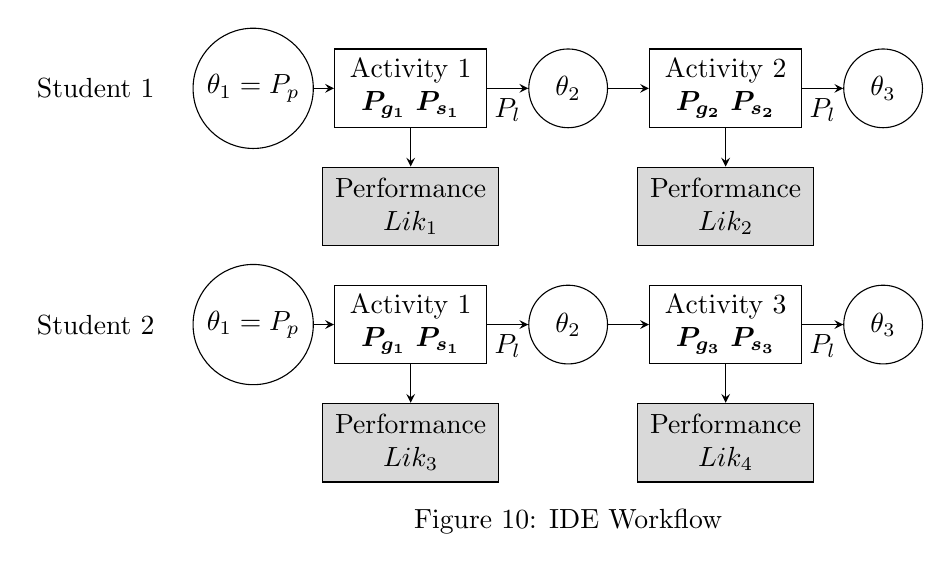
\begin{tikzpicture}
        % Define styles
        \tikzset{
            state/.style={circle, draw, minimum size=1cm},
            activity/.style={rectangle, draw, minimum size=1cm},
            performance/.style={rectangle, draw, fill=gray!30, minimum size=1cm},
            arrow/.style={->,>=stealth}
        }
        
        % Nodes
        \node[] () at (-2,0) {Student 1};
        \node[state] (state_node_1) at (0,0) {$\theta_1 = P_p$};
        \node[activity] (activity_node_1) at (2,0) {\parbox{1.7cm}{\centering Activity 1 \\ $\boldsymbol{P_{g_1} \ P_{s_1}}$}};
        \node[performance] (performance_node_1) at (2,-1.5) {\parbox{2cm}{\centering Performance \\ $Lik_1$}};
        \node[state] (state_node_2) at (4,0) {$\theta_2$};
        
        \node[activity] (activity_node_2) at (6,0) {\parbox{1.7cm}{\centering Activity 2 \\ $\boldsymbol{P_{g_2} \ P_{s_2}}$}};
        \node[performance] (performance_node_2) at (6,-1.5) {\parbox{2cm}{\centering Performance \\ $Lik_2$}};
        \node[state] (state_node_3) at (8,0) {$\theta_3$};
        
        % Arrows
        \draw[arrow] (state_node_1) -- (activity_node_1);
        \draw[arrow] (activity_node_1) -- (state_node_2) node[midway, below] {$P_l$};
        \draw[arrow] (activity_node_1) -- (performance_node_1);
        \draw[arrow] (state_node_2) -- (activity_node_2);
        \draw[arrow] (activity_node_2) -- (state_node_3) node[midway, below] {$P_l$};
        \draw[arrow] (activity_node_2) -- (performance_node_2);
    

        % student 2
        \node[] () at (-2,-3) {Student 2};
        \node[state] (state_node_2) at (0,-3) {$\theta_1 = P_p$};
        \node[activity] (activity_node_2) at (2,-3) {\parbox{1.7cm}{\centering Activity 1 \\ $\boldsymbol{P_{g_1} \ P_{s_1}}$}};
        \node[performance] (performance_node_2) at (2,-4.5) {\parbox{2cm}{\centering Performance \\ $Lik_3$}};
        \node[state] (state_node_3) at (4,-3) {$\theta_2$};
        \node[activity] (activity_node_3) at (6,-3) {\parbox{1.7cm}{\centering Activity 3 \\ $\boldsymbol{P_{g_3} \ P_{s_3}}$}};
        \node[performance] (performance_node_3) at (6,-4.5) {\parbox{2cm}{\centering Performance \\ $Lik_4$}};
        \node[state] (state_node_4) at (8,-3) {$\theta_3$};
        \draw[arrow] (state_node_2) -- (activity_node_2);
        \draw[arrow] (activity_node_2) -- (state_node_3) node[midway, below] {$P_l$};
        \draw[arrow] (activity_node_2) -- (performance_node_2);
        \draw[arrow] (state_node_3) -- (activity_node_3);
        \draw[arrow] (activity_node_3) -- (state_node_4) node[midway, below] {$P_l$};
        \draw[arrow] (activity_node_3) -- (performance_node_3);

        % Footnote
        \node at (4,-5.5) {Figure 10: IDE Workflow};
    \end{tikzpicture}
\end{center}


\subsubsection{Forget}

The learning and forgetting behavior (LFB) Model (\cite{forget}) is based on BKT that consider forgetting as part of learning process. The LFB assumes that 

The main difference in the model description lies in the state changes.Besides original three types of learning state changes (Remaining Known, Learning, Remaining Unknown), LFB adds Forget which is illustrated in Figure 11.

\begin{center}
    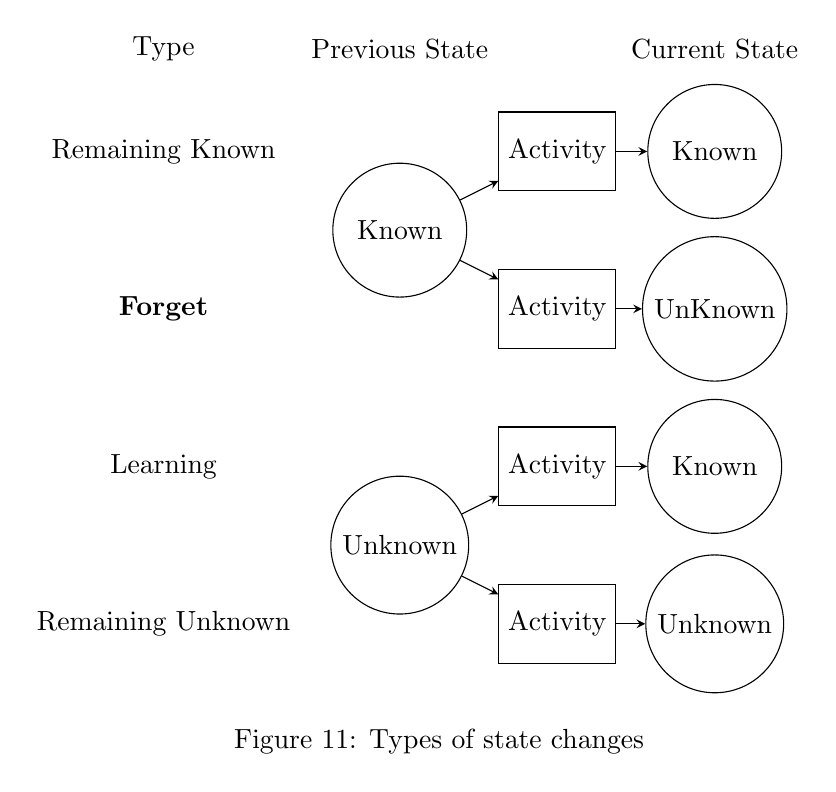
\begin{tikzpicture}
        % Define styles
        \tikzset{
            state/.style={circle, draw, minimum size=1.7cm},
            activity/.style={rectangle, draw, minimum size=1cm},
            arrow/.style={->,>=stealth}
        }
        
        % Nodes
        \node[] () at (-3,3.3) {Type};
        \node[] () at (0,3.3) {Previous State};
        \node[] () at (4,3.3) {Current State};

        \node[] () at (-3,2) {Remaining Known};
        \node[state] (state_node_1) at (0,1) {Known};
        \node[activity] (activity_node_1) at (2,2) {Activity};
        \node[state] (state_node_2) at (4,2) {Known};

        \node[] () at (-3,0) {\textbf{Forget}};
        \node[activity] (activity_node_0) at (2,0) {Activity};
        \node[state] (state_node_0) at (4,0) {UnKnown};
        
        \node[] () at (-3,-2) {Learning};
        \node[state] (state_node_3) at (0,-3) {Unknown};
        \node[activity] (activity_node_2) at (2,-2) {Activity};
        \node[state] (state_node_4) at (4,-2) {Known};
        
        \node[] () at (-3,-4) {Remaining Unknown};
        % \node[state] (state_node_5) at (0,-4) {Unknown};
        \node[activity] (activity_node_3) at (2,-4) {Activity};
        \node[state] (state_node_6) at (4,-4) {Unknown};
        
        % Arrows
        \draw[arrow] (state_node_1) -- (activity_node_1);
        \draw[arrow] (state_node_1) -- (activity_node_0);
        \draw[arrow] (activity_node_1) -- (state_node_2);
        \draw[arrow] (activity_node_0) -- (state_node_0);
        \draw[arrow] (state_node_3) -- (activity_node_2);
        \draw[arrow] (activity_node_2) -- (state_node_4);
        \draw[arrow] (state_node_3) -- (activity_node_3);
        \draw[arrow] (activity_node_3) -- (state_node_6);
    
        % Footnote
        \node at (0.5,-5.5) {Figure 11: Types of state changes};
    \end{tikzpicture}
\end{center}

In LFB terminology, we add the following defines:

1. \textbf{Forget}  
The forget rate, \( P_f \), represents the probability that a learner transitions to the unknown state through forgetting.

LFB Updates \(\theta_{i+1}\) by incorporating the potential learning effect based on \(\theta'\) in a different way with BKT, considering the effect of forget change.

$$
\theta_{i+1} = \theta' \boldsymbol{P_f} + (1 - \theta') P_l    
$$

The workflow of LFB is illustrated in Figure 12. Note there are forget parameters $P_f$ in use.

\begin{center}
    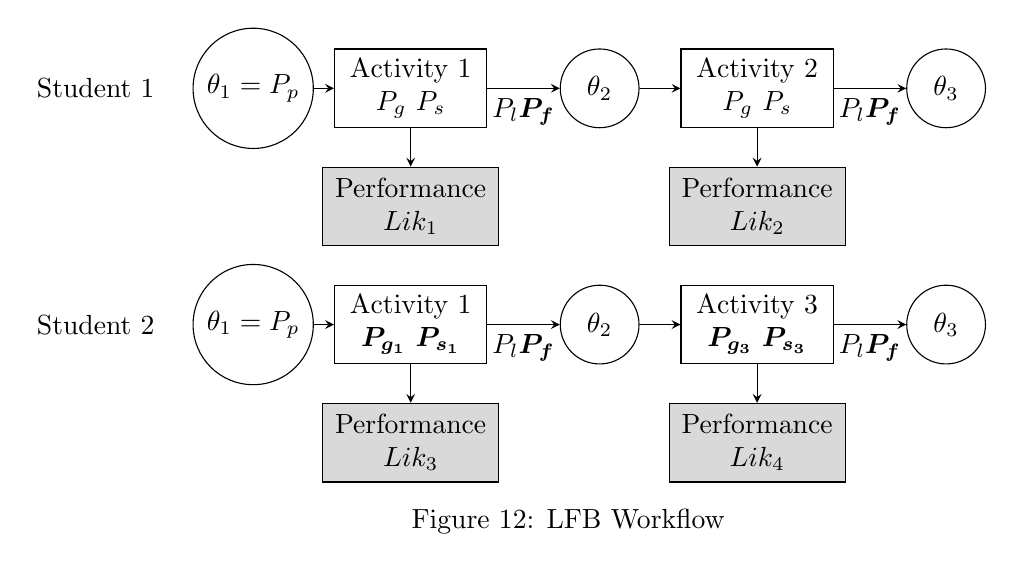
\begin{tikzpicture}
        % Define styles
        \tikzset{
            state/.style={circle, draw, minimum size=1cm},
            activity/.style={rectangle, draw, minimum size=1cm},
            performance/.style={rectangle, draw, fill=gray!30, minimum size=1cm},
            arrow/.style={->,>=stealth}
        }
        
        % Nodes
        \node[] () at (-2,0) {Student 1};
        \node[state] (state_node_1) at (0,0) {$\theta_1 = P_p$};
        \node[activity] (activity_node_1) at (2,0) {\parbox{1.7cm}{\centering Activity 1 \\ ${P_{g} \ P_{s}}$}};
        \node[performance] (performance_node_1) at (2,-1.5) {\parbox{2cm}{\centering Performance \\ $Lik_1$}};
        \node[state] (state_node_2) at (4.4,0) {$\theta_2$};
        
        \node[activity] (activity_node_2) at (6.4,0) {\parbox{1.7cm}{\centering Activity 2 \\ ${P_{g} \ P_{s}}$}};
        \node[performance] (performance_node_2) at (6.4,-1.5) {\parbox{2cm}{\centering Performance \\ $Lik_2$}};
        \node[state] (state_node_3) at (8.8,0) {$\theta_3$};
        
        % Arrows
        \draw[arrow] (state_node_1) -- (activity_node_1);
        \draw[arrow] (activity_node_1) -- (state_node_2) node[midway, below] {$P_l \boldsymbol{P_f}$};
        \draw[arrow] (activity_node_1) -- (performance_node_1);
        \draw[arrow] (state_node_2) -- (activity_node_2);
        \draw[arrow] (activity_node_2) -- (state_node_3) node[midway, below] {$P_l \boldsymbol{P_f}$};
        \draw[arrow] (activity_node_2) -- (performance_node_2);
    

        % student 2
        \node[] () at (-2,-3) {Student 2};
        \node[state] (state_node_2) at (0,-3) {$\theta_1 = P_p$};
        \node[activity] (activity_node_2) at (2,-3) {\parbox{1.7cm}{\centering Activity 1 \\ $\boldsymbol{P_{g_1} \ P_{s_1}}$}};
        \node[performance] (performance_node_2) at (2,-4.5) {\parbox{2cm}{\centering Performance \\ $Lik_3$}};
        \node[state] (state_node_3) at (4.4,-3) {$\theta_2$};
        \node[activity] (activity_node_3) at (6.4,-3) {\parbox{1.7cm}{\centering Activity 3 \\ $\boldsymbol{P_{g_3} \ P_{s_3}}$}};
        \node[performance] (performance_node_3) at (6.4,-4.5) {\parbox{2cm}{\centering Performance \\ $Lik_4$}};
        \node[state] (state_node_4) at (8.8,-3) {$\theta_3$};
        \draw[arrow] (state_node_2) -- (activity_node_2);
        \draw[arrow] (activity_node_2) -- (state_node_3) node[midway, below] {$P_l \boldsymbol{P_f}$};
        \draw[arrow] (activity_node_2) -- (performance_node_2);
        \draw[arrow] (state_node_3) -- (activity_node_3);
        \draw[arrow] (activity_node_3) -- (state_node_4) node[midway, below] {$P_l \boldsymbol{P_f}$};
        \draw[arrow] (activity_node_3) -- (performance_node_3);

        % Footnote
        \node at (4,-5.5) {Figure 12: LFB Workflow};
    \end{tikzpicture}
\end{center}
\section{Estimation}

To estimate the global parameters of the BKT model (\(P_p, P_l, P_s, P_g\)) that maximize the likelihood \(Lik\), we employ the expectation-maximization (EM) algorithm. This algorithm is particularly well-suited for the BKT model as it addresses the latent nature of the learner's knowledge state (\(\theta_i\)), which cannot be directly observed but significantly influences the observed responses.

The EM algorithm consists of two iterative steps: the Expectation (E-step) and the Maximization (M-step). These steps are repeated until convergence. An overview of the algorithm is in Algorithm \ref{al:1}.

\begin{algorithm}

\caption{EM Algorithm for BKT Parameter Estimation}
\begin{algorithmic}[1]
\STATE \textbf{Input:} Observed answers \(a_i\) for each learner
\STATE \textbf{Output:} Estimated parameters \(P_p, P_l, P_s, P_g\)
\STATE Initialize parameters \(P_p, P_l, P_s, P_g\)
\STATE \textbf{Repeat until convergence:}
    \STATE \quad \textbf{E-step:}
    \STATE \quad \quad For each learner \(j\):
    \STATE \quad \quad \quad Update \(\theta_i\) using Bayes' rule and incorporate learning
    \STATE \quad \quad \quad Compute likelihood \(Lik_i\) for each answer \(a_i\)
    \STATE \quad \quad \quad Accumulate likelihood to total \(Lik\)
    \STATE \quad \textbf{M-step:}
    \STATE \quad \quad Update \(P_p, P_l, P_s, P_g\) based on expectations from E-step
\STATE \textbf{Until convergence (change in \(\log Lik\) below threshold)}
\end{algorithmic}
\label{al:1}
\end{algorithm}

\subsection{E-step}
In the E-step, we calculate the expected values of the latent knowledge state (\(\theta_i\)) and the associated contributions to the likelihood based on the current estimates of the global parameters. Specifically, for each learner:

1. \textbf{Initialization}:
Set the initial knowledge state \(\theta_1 = P_p\).

2. \textbf{Forward Computation}:
For each activity \(i\) in the sequence, iteratively compute the known rate \(\theta_{i+1}\):

- First, update the known rate \(\theta'\) based on the observed answer \(a_i\) using Bayes' rule:
\[
\theta' = 
\begin{cases} 
    \frac{\theta_i P_s}{\theta_i P_s + (1 - \theta_i)(1 - P_g)}, & \text{if } a_i = 0 \\
    \frac{\theta_i (1 - P_s)}{\theta_i (1 - P_s) + (1 - \theta_i)P_g}, & \text{if } a_i = 1
\end{cases}
\]

- Then incorporate the learning effect to compute \(\theta_{i+1}\):
\[
\theta_{i+1} = \theta' + (1 - \theta')P_l
\]

3. \textbf{Likelihood Contribution}:
Compute the likelihood for each observed answer \(a_i\):
\[
Lik_i = 
\begin{cases} 
    P_s \theta_i + (1 - P_g)(1 - \theta_i), & \text{if } a_i = 0 \\
    (1 - P_s)\theta_i + P_g(1 - \theta_i), & \text{if } a_i = 1
\end{cases}
\]
Accumulate these likelihoods to update the total likelihood \(Lik\).

\subsection{M-step}
In the M-step, we maximize the expected likelihood with respect to the global parameters (\(P_p, P_l, P_s, P_g\)). This involves:

1. \textbf{Updating Prior (\(P_p\))}:

    The prior probability \(P_p\) is updated based on the expected initial knowledge state \(\theta_1\):
    \[
    P_p = \frac{1}{N} \sum_{j=1}^N \theta_1^{(j)},
    \]
    where \(N\) is the total number of learners, and \(\theta_1^{(j)}\) is the initial knowledge state of learner \(j\).

2. \textbf{Updating Learning Rate (\(P_l\))}:

    The learning rate \(P_l\) is updated based on the transitions from \(\theta'\) (updated state after observing \(a_i\)) to \(\theta_{i+1}\):
    \[
    P_l = \frac{\sum_{j=1}^N \sum_{i=1}^{T_j} \left( (1 - \theta_i^{(j)}) \cdot \theta_{i+1}^{(j)} \right)}{\sum_{j=1}^N \sum_{i=1}^{T_j} (1 - \theta_i^{(j)})},
    \]
    where \(T_j\) is the number of activities for learner \(j\).

3. \textbf{Updating Slip Rate (\(P_s\))}:

    The slip rate \(P_s\) is updated based on the proportion of incorrect answers when the learner is in the known state:
    \[
    P_s = \frac{\sum_{j=1}^N \sum_{i=1}^{T_j} \left( \theta_i^{(j)} \cdot (1 - a_i) \right)}{\sum_{j=1}^N \sum_{i=1}^{T_j} \theta_i^{(j)}},
    \]

4. \textbf{Updating Guess Rate (\(P_g\))}:

    The guess rate \(P_g\) is updated based on the proportion of correct answers when the learner is in the unknown state:
    \[
    P_g = \frac{\sum_{j=1}^N \sum_{i=1}^{T_j} \left( (1 - \theta_i^{(j)}) \cdot a_i \right)}{\sum_{j=1}^N \sum_{i=1}^{T_j} (1 - \theta_i^{(j)})},
    \]

\subsection{Iteration and Convergence}
The E-step and M-step are alternated until the likelihood \(Lik\) converges, i.e., when the change in \(\log Lik\) between iterations falls below a predefined threshold. At convergence, the global parameters (\(P_p, P_l, P_s, P_g\)) maximize the likelihood of the observed answer sequences under the BKT model.

By iteratively refining the parameter estimates and leveraging the hidden knowledge state dynamics, the EM algorithm ensures an efficient and robust estimation process for the BKT model.   


\subsection{ILE Estimation}

In the Item Learning Effect (ILE) model, the primary modification to the standard BKT model is the individualization of the learning rate for each activity. Instead of a global learning rate \( P_l \), the ILE model assigns a unique learning rate \( P_{l_j} \) for each item \( j \). To estimate the global parameters (\( P_p, P_{l_j}, P_s, P_g \)) that maximize the likelihood of the observed responses, we extend the Expectation-Maximization (EM) algorithm to handle the item-specific learning rates.



The estimation procedure for the ILE model follows similar steps as the standard BKT model but includes modifications for handling the different learning rates for each item.

\subsubsection{E-step}

\begin{enumerate}
    \item \textbf{Initialization}:
    Set the initial knowledge state \(\theta_1 = P_p\), as in the basic BKT model.
    
    \item \textbf{Forward Computation}:
    For each activity \(i\) in the sequence, compute the updated knowledge state \(\theta'\) using Bayes' rule, with the learning rate \(P_{l_i}\) specific to activity \(i\):
    \[
    \theta' = 
    \begin{cases} 
        \frac{\theta_i P_s}{\theta_i P_s + (1 - \theta_i)(1 - P_g)}, & \text{if } a_i = 0 \\
        \frac{\theta_i (1 - P_s)}{\theta_i (1 - P_s) + (1 - \theta_i)P_g}, & \text{if } a_i = 1
    \end{cases}
    \]
    
    Then, update the knowledge state \(\theta_{i+1}\) for each learner based on the individual learning rate \(P_{l_i}\) for activity \(i\):
    \[
    \theta_{i+1} = \theta' + (1 - \theta') P_{l_i}
    \]
    
    \item \textbf{Likelihood Contribution}:
    For each observed answer \(a_i\) at activity \(i\), the likelihood contribution is computed as:
    \[
    Lik_i = 
    \begin{cases} 
        P_s \theta_i + (1 - P_g)(1 - \theta_i), & \text{if } a_i = 0 \\
        (1 - P_s)\theta_i + P_g(1 - \theta_i), & \text{if } a_i = 1
    \end{cases}
    \]
    The likelihoods are accumulated to update the total likelihood \(Lik\).
\end{enumerate}

\subsubsection{M-step}
In the M-step, we maximize the expected likelihood computed during the E-step with respect to the global parameters (\(P_p, P_{l_j}, P_s, P_g\)).

\begin{enumerate}
    \item \textbf{Updating Prior (\(P_p\))}:
    The prior probability \(P_p\) is updated based on the expected initial knowledge state \(\theta_1\), as in the basic BKT model:
    \[
    P_p = \frac{1}{N} \sum_{j=1}^N \theta_1^{(j)}
    \]

    \item \textbf{Updating Item-Specific Learning Rate (\(P_{l_j}\))}:
    The learning rate for each item \(j\), \(P_{l_j}\), is updated based on the transitions from the knowledge state after observing the learner's answers for that activity:
    \[
    P_{l_j} = \frac{\sum_{j=1}^N \sum_{i=1}^{T_j} \left( (1 - \theta_i^{(j)}) \cdot \theta_{i+1}^{(j)} \right)}{\sum_{j=1}^N \sum_{i=1}^{T_j} (1 - \theta_i^{(j)})}
    \]
    Here, \(T_j\) refers to the number of activities for learner \(j\), and each item-specific learning rate \(P_{l_j}\) is calculated independently for each activity.

    \item \textbf{Updating Slip Rate (\(P_s\))}:
    The slip rate \(P_s\) is updated based on the proportion of incorrect answers when the learner is in the known state across all items:
    \[
    P_s = \frac{\sum_{j=1}^N \sum_{i=1}^{T_j} \left( \theta_i^{(j)} \cdot (1 - a_i) \right)}{\sum_{j=1}^N \sum_{i=1}^{T_j} \theta_i^{(j)}}
    \]

    \item \textbf{Updating Guess Rate (\(P_g\))}:
    The guess rate \(P_g\) is updated based on the proportion of correct answers when the learner is in the unknown state across all items:
    \[
    P_g = \frac{\sum_{j=1}^N \sum_{i=1}^{T_j} \left( (1 - \theta_i^{(j)}) \cdot a_i \right)}{\sum_{j=1}^N \sum_{i=1}^{T_j} (1 - \theta_i^{(j)})}
    \]
\end{enumerate}

\subsubsection{Iteration and Convergence}
The E-step and M-step are alternated until convergence, similar to the basic BKT model. The algorithm converges when the change in the log-likelihood between iterations is below a predefined threshold. At this point, the estimated parameters (\(P_p, P_{l_j}, P_s, P_g\)) maximize the likelihood of the observed sequences of answers under the ILE model.

\subsubsection{Summary}
In the ILE model, the primary difference from the standard BKT model is the individualization of the learning rate for each activity. The EM algorithm is extended to estimate the item-specific learning rates \(P_{l_j}\) along with the other parameters. This allows for a more fine-grained representation of how learners progress through different items.


\section{Simulation}

This section describes the synthetic dataset generation process following the basic BKT model.

\subsection{Data Generation Workflow}
The data generation follows these key steps, corresponding to the abstraction of the learning process described in the \textbf{Model Description} part.


\begin{enumerate}
    \item \textbf{Student Initialization}: Each student begins with:
    \begin{itemize}
        \item Initial know state $k_1 \sim \text{Bernoulli}(P_p)$
        \item Initialize the number of activities for the student, $T_{max} \sim \text{Uniform}(1, 10)$, where $T_{max}$ is an integer uniformly sampled from 1 to 10.
    \end{itemize}
    
    \item \textbf{Activity-Performing Process}:
    \begin{itemize}
        \item For each activity $t \in [1, T_{\text{max}}]$:
        \begin{itemize}
            \item If unmastered ($k_t=0$): $p_{\text{correct}} = guess$
            \item If mastered ($k_t=1$): $p_{\text{correct}} = 1-slip$
            \item Generate response $correct_t \sim \text{Bernoulli}(p_{\text{correct}})$
        \end{itemize}
    \end{itemize}
    
    \item \textbf{Knowledge State Update}:
    \begin{itemize}
        \item After each attempt: $k_{t+1} \sim \text{Bernoulli}(learn)$ if $k_t=0$
        \item Persistent mastery once $k_t=1$
    \end{itemize}
    
    \item \textbf{Dataset Assembly}:
    \begin{itemize}
        \item Collect records with columns: 
        \begin{itemize}
            \item \texttt{order\_id}, \texttt{correct}, \texttt{student\_id}
        \end{itemize}
    \end{itemize}
\end{enumerate}

\subsection{Example of Generated Data}

The following is a preview of the structure of the generated dataset:

\begin{table}[ht]
\centering
\caption{Example of Simulated Data}
\label{tab:example-data}
\begin{tabular}{|c|c|c|}
\hline
\textbf{order\_id} & \textbf{correct} & \textbf{student\_id} \\ \hline
1 & 0 & 1 \\ \hline
2 & 0 & 1 \\ \hline
3 & 1 & 1 \\ \hline
... & ... & ... \\ \hline
11 & 0 & 2 \\ \hline
12 & 0 & 2 \\ \hline
13 & 0 & 2 \\ \hline
... & ... & ... \\ \hline
\end{tabular}
\end{table}

\subsection{Simulation Parameters}
Three datasets were generated using the parameters in Table~\ref{tab:sim_params} to evaluate scalability.

\begin{table}[H]
\centering
\caption{BKT Simulation Parameters and Values}
\label{tab:sim_params}
\begin{tabular}{@{}lll@{}}
\toprule
\textbf{Parameter} & \textbf{Value(s)} & \textbf{Description} \\
\midrule
\texttt{prior} & 0.2 & Initial mastery probability \\
\texttt{guess} & 0.1 & Guess probability \\
\texttt{slip} & 0.1 & Slip probability \\
\texttt{learn} & 0.3 & Learning probability \\
\texttt{num\_students} & 50, 500, 2000 & Dataset sizes \\
\texttt{max\_questions} & 10 & Maximum questions per student \\
\bottomrule
\end{tabular}
\end{table}

\subsection{Comparison Result}
The generated simulation data was used to fit the basic BKT model in both the \texttt{BKT} and \texttt{pyBKT} packages. The results of the fitting process are shown in Table \ref{tab:bkt-comparison}.
\begin{table}[H]
\centering
\caption{Comparison of BKT and pyBKT Results}
\label{tab:bkt-comparison}
\begin{tabular}{@{}clccc@{}}
\toprule
\textbf{Data Size} & \textbf{Parameter} & \textbf{Origin Value} & \textbf{BKT Value} & \textbf{pyBKT Value} \\
\midrule
\multirow{4}{*}{50} 
    & Prior   & 0.2 & 0.261569 & 0.25647 \\
    & Learn   & 0.3 & 0.374822 & 0.32318 \\
    & Guess   & 0.1 & 0.093822 & 0.08976 \\
    & Slip    & 0.1 & 0.111001 & 0.12422 \\
\midrule
\multirow{4}{*}{500} 
    & Prior   & 0.2 & 0.232586 & 0.22841 \\
    & Learn   & 0.3 & 0.296199 & 0.28833 \\
    & Guess   & 0.1 & 0.092990 & 0.09644 \\
    & Slip    & 0.1 & 0.088352 & 0.08931 \\
\midrule
\multirow{4}{*}{2000} 
    & Prior   & 0.2 & 0.196425 & 0.19982 \\
    & Learn   & 0.3 & 0.304423 & 0.29789 \\
    & Guess   & 0.1 & 0.103813 & 0.10712 \\
    & Slip    & 0.1 & 0.102593 & 0.09861 \\
\bottomrule
\end{tabular}
\end{table}
\subsection{MSE and Bias}

Table~\ref{tab:sim_params_3} presents the Mean Squared Error (MSE) and Bias for different dataset sizes (50, 500, and 2000 students) in the estimation of the four parameters: \textit{Learns}, \textit{Guesses}, \textit{Slips}, and \textit{Prior}.

\begin{table}[H]
\centering
\caption{BKT Simulation Parameters for Different Settings}
\label{tab:sim_params_3}
\begin{tabular}{@{}lcc@{}}
\toprule
\textbf{Parameter} & \textbf{Setting A} & \textbf{Setting B} \\ 
\midrule
\texttt{prior} & 0.2 & 0.0 \\ 
\texttt{guess} & 0.03 & 0.5 \\ 
\texttt{slip} & 0.01 & 0.05 \\ 
\texttt{learn} & 0.2 & 0.3 \\ 
\texttt{num\_students} & 50, 500, 2000 & 50, 500, 2000 \\ 
\texttt{max\_questions} & 10 & 10 \\ 
\bottomrule
\end{tabular}
\end{table}
    
The MSE values quantify the average squared differences between the estimated and origin values, while Bias indicates the systematic deviation of the estimates. Here, the origin values refer to the parameters used to generate the simulated data, rather than the true values of the generated data. Due to the stochastic nature of the data generation process, the parameters of the generated data are not guaranteed to be exactly equal to the specified origin values.

To account for this variability, we conducted 100 simulation runs and computed the average MSE and Bias values. The results are presented in Table~\ref{tab:mse-bias-comparison}.
\begin{table}[H]
\centering
\caption{MSE and Bias}
\label{tab:mse-bias-comparison}
\begin{tabular}{@{}cclcccc@{}}
\toprule
\textbf{Data Size} & \textbf{Setting} & \textbf{Metric} & \texttt{learns} & \texttt{guesses} & \texttt{slips} & \texttt{prior} \\ 
\midrule
\multirow{4}{*}{50}  
    & A & MSE  & 0.002073 & 0.000393 & 0.000104 & 0.003834 \\  
    & B & MSE  & 0.010618 & 0.009161 & 0.001365 & 0.020640 \\  
    & A & Bias & 0.006589 & -0.000646 & -0.000269 & 0.000453 \\  
    & B & Bias & 0.035441 & -0.054509 & 0.012494 & 0.091014 \\  
\midrule
\multirow{4}{*}{500}  
    & A & MSE  & 0.000168 & 0.000043 & 0.000013 & 0.000311 \\  
    & B & MSE  & 0.000711 & 0.000743 & 0.000119 & 0.001798 \\  
    & A & Bias & -0.000109 & 0.000527 & 0.000636 & -0.000490 \\  
    & B & Bias & 0.005335 & -0.012432 & 0.002067 & 0.029230 \\  
\midrule
\multirow{4}{*}{2000}  
    & A & MSE  & 0.000037 & 0.000008 & 0.000003 & 0.000080 \\  
    & B & MSE  & 0.000174 & 0.000195 & 0.000036 & 0.000676 \\  
    & A & Bias & 0.001181 & -0.000250 & -0.000160 & -0.000114 \\  
    & B & Bias & -0.000320 & -0.008643 & 0.001474 & 0.020545 \\  
\bottomrule
\end{tabular}
\end{table}

\section{Data Example}

The dataset originates from the Cognitive Tutor system (\cite{ritter2007cognitive}), an intelligent tutoring platform designed to enhance students' mathematical abilities. This platform has been utilized extensively to capture detailed logs of student interactions during math problem-solving activities.

The dataset comprises detailed logs of 587 unique students' interactions with Cognitive Tutor, tracking their responses to a series of mathematical problems related to various Knowledge Components (KCs). Overall, the dataset contains 16,857 observation records that detail each student's attempts and the correctness of their responses across these 12 KCs.

The primary goal of this dataset is to facilitate a deeper understanding of the processes through which students learn mathematics and to enhance their learning outcomes based on this understanding. Furthermore, this data allows researchers to explore and quantify patterns in student learning behaviors and how these are influenced by tasks, hints, and feedback patterns integrated within the Cognitive Tutor system.

In addition to the descriptive analysis of the dataset, this paper also involves preprocessing the data to meet the input requirements of the Bayesian Knowledge Tracing (BKT) model. Specifically, the preprocessing step will transform the data by sequencing each student's responses to the math problems. This will be structured as a chronological sequence of attempts for each student, where each attempt is marked by their response correctness. This sequence forms a crucial input for the BKT model, enabling it to trace and predict the evolution of each student's knowledge state over time.

\subsection{Basic BKT Model Example with BKT R package}

\begin{lstlisting}[caption={R code to train a simple BKT model}]
library(BKT)

# Initialize the model with an optional seed
model <- bkt(seed = 42, num_fits = 1, parallel = FALSE)

# Fetch example data
fetch_dataset(model, "https://raw.githubusercontent.com/CAHLR/pyBKT-examples/master/data/ct.csv", ".")

# Train a simple BKT model on one skill in the CT dataset
result <- fit(model, data_path = "ct.csv", skills = "Plot non-terminating improper fraction")

# View the trained parameters
print(params(result))
\end{lstlisting}

The result will be shown as below: 

\begin{verbatim}
    skill                                 param  class   value
1 Plot non-terminating improper fraction  learns default 0.222837
2 Plot non-terminating improper fraction guesses default 0.002951
3 Plot non-terminating improper fraction   slips default 0.322440
4 Plot non-terminating improper fraction   prior default 0.737934
\end{verbatim}

In the result, the first column is the name of the skills, the second column indicates the type of parameters, including \texttt{learns}, \texttt{forgets}, \texttt{guesses}, \texttt{slips}, and \texttt{prior}. The last column shows the estimated parameter value.

Learns (0.222808): This parameter indicates the probability that a student will transition from the "not learned" state to the "learned" state after completing an attempt. In this example, the probability of learning from an attempt is approximately 22.3\%, suggesting moderate learning potential.

Guesses (0.003382): This parameter estimates the likelihood that a student who has not mastered the skill can guess the correct answer. A very low value (0.3\%) here indicates that guessing correctly is highly unlikely for this skill.

Slips (0.322177): This parameter represents the probability that a student who has already mastered the skill will provide an incorrect answer. The value of 32.2\% suggests a relatively high chance of error due to slips, which may occur due to distractions, miscalculations, or other external factors.

Prior (0.737443): The prior parameter indicates the initial probability of a student knowing the skill before interacting with the tutor. Here, approximately 73.7\% of students are estimated to already possess this knowledge, reflecting a relatively high prior knowledge for this specific skill.

\subsection{PPS BKT Model Example with BKT R package}

Train a multiple prior BKT model for multiple students in the CT dataset. Switch parameter \texttt{multiprior = TRUE} in the \texttt{fit} function.

Multiple Prior refers to the Prior Per Student (PPS) Model.

\begin{lstlisting}[caption={R code to train a PPS BKT model}]
library(BKT)

# Initialize the model with an optional seed
model <- bkt(seed = 42, num_fits = 10, parallel = FALSE)

# Fetch example data
fetch_dataset(model, "https://raw.githubusercontent.com/CAHLR/pyBKT-examples/master/data/ct.csv", ".")

# Train a multiple guess BKT model on one skill in the CT dataset
result <- fit(model, data_path = "ct.csv", skills = c("Finding the intersection, Mixed"), multiprior = TRUE)

# View the trained parameters
print(params(result))
\end{lstlisting}

The result will be shown as below:

\begin{verbatim}
    skill                           param        class    value
1  Finding the intersection, Mixed  learns      default 0.016332
2  Finding the intersection, Mixed guesses      default 0.292058
3  Finding the intersection, Mixed   slips      default 0.240662
4  Finding the intersection, Mixed   prior     171eKI1Z 1.000000
5  Finding the intersection, Mixed   prior     171nKnHW 1.000000
6  Finding the intersection, Mixed   prior     171RUh1Q 1.000000
7  Finding the intersection, Mixed   prior      1T4w47X 0.000000
...
76 Finding the intersection, Mixed   prior      3cjD21W 1.000000
77 Finding the intersection, Mixed   prior      Vd9xmeb 1.000000
\end{verbatim}
    
Note that the \texttt{class} column refers to different students.

Learns (0.016332): This parameter represents the probability that a student transitions from the "not learned" to the "learned" state after an attempt. In this case, the value of 0.016332 is relatively low, which suggests that the skill "Finding the intersection, Mixed" is not easily learned after just a single attempt, requiring more practice and interaction for the student to gain mastery.

Guesses (0.292058) The guesses parameter indicates the likelihood that a student, despite not mastering the skill, can guess the correct answer. With a value of 0.292058, this suggests a moderate probability of correct guesses for this skill. This implies that students have a reasonable chance of answering the question correctly even without mastering the skill, possibly due to the nature of the task or its clues.

Slips (0.240662): The slips parameter shows the probability that a student who has already mastered the skill will provide an incorrect answer. The value of 0.240662 suggests that there is a moderate likelihood of errors (or slips) occurring despite mastery. This could be attributed to factors such as fatigue, distractions, or misinterpretation of the question.

Prior (varied for individual students): The prior parameters are individualized for each student in the PPS model, as seen in the dataset. The prior values for different students range from 0 to 1, indicating the estimated prior knowledge each student possesses before interacting with the tutor. The prior for each student is labeled uniquely (e.g., 171eKI1Z, 171nKnHW, etc.), representing the varying degrees of prior knowledge across the student population. A majority of the priors are close to 1, meaning that many students are estimated to have a high level of prior knowledge for the skill before they start interacting with the tutor. However, some students (e.g., 1T4w47X) have a prior value closer to 0, indicating that they have little to no prior knowledge of the skill at the beginning of the tutoring process.

\subsection{IDE BKT Model Example with BKT R package}

Train a multiple guess and slip BKT model on multiple skills in the CT dataset. Switch parameter \texttt{multigs = TRUE} in the \texttt{fit} function.

Multiple Guess refers to the Item Difficulty Effect (IDE) Model.

\begin{lstlisting}[caption={R code to train an ILE BKT model}]
library(BKT)

# Initialize the model with an optional seed
model <- bkt(seed = 42, num_fits = 10, parallel = FALSE)

# Fetch example data
fetch_dataset(model, "https://raw.githubusercontent.com/CAHLR/pyBKT-examples/master/data/ct.csv", ".")

# Train a multiple guess BKT model on one skill in the CT dataset
result <- fit(model, data_path = "ct.csv", skills = c("Finding the intersection, Mixed"), multigs = TRUE)

# View the trained parameters
print(params(result))
\end{lstlisting}

The result will be shown as below:

\begin{verbatim}
                             skill   param                class    value
1  Finding the intersection, Mixed  learns              default 0.004373
2  Finding the intersection, Mixed guesses   M2X-4Y=18&Y=-3X+13 0.331227
3  Finding the intersection, Mixed guesses M2X-4YGT18&YLE-3X+13 1.000000
...
17 Finding the intersection, Mixed guesses            SY=-X&Y=7 0.000000
18 Finding the intersection, Mixed   slips   M2X-4Y=18&Y=-3X+13 0.000000
19 Finding the intersection, Mixed   slips M2X-4YGT18&YLE-3X+13 0.00000
...
33 Finding the intersection, Mixed   slips            SY=-X&Y=7 0.058531
34 Finding the intersection, Mixed   prior              default 0.851380
\end{verbatim}
    
Note that the \texttt{class} column refers to different items.

Learns (0.004373): This parameter represents the probability of a student transitioning from the "not learned" to the "learned" state after an attempt. A very low value of 0.004373 indicates that the skill "Finding the intersection, Mixed" is challenging to learn, requiring multiple attempts for students to acquire proficiency.

Guesses (varies by class): The guesses parameter varies significantly across the 16 item difficulty classes, highlighting how the probability of correctly guessing depends on the difficulty level of the question.

Slips (varies by class): The slips parameter also varies across classes, representing the likelihood of a student making an error despite mastering the skill.

Prior (0.851380): The prior probability of 0.851 indicates that 85.13\% of students are estimated to have already mastered the "Finding the intersection, Mixed" skill before interacting with the tutor. This reflects a high level of initial knowledge among the students for this specific skill.

\subsection{ILE BKT Model Example with BKT R package}

Train a multiple learn BKT model on multiple skills in the CT dataset. Switch parameter \texttt{multilearn = TRUE} in the \texttt{fit} function.

Multiple Learn refers to the Item Learning Effect (ILE) Model.

\begin{lstlisting}[caption={R code to train an ILE BKT model}]
library(BKT)

# Initialize the model with an optional seed
model <- bkt(seed = 42, num_fits = 10, parallel = FALSE)

# Fetch example data
fetch_dataset(model, "https://raw.githubusercontent.com/CAHLR/pyBKT-examples/master/data/ct.csv", ".")

# Train a multiple guess BKT model on one skill in the CT dataset
result <- fit(model, data_path = "ct.csv", skills = c("Finding the intersection, Mixed"), multilearn = TRUE)

# View the trained parameters
print(params(result))
\end{lstlisting}

The result will be shown as below:

\begin{verbatim}
    skill                           param              class    value
1  Finding the intersection, Mixed  learns   M2X-4Y=18&Y=-3X+13 0.000000
2  Finding the intersection, Mixed  learns M2X-4YGT18&YLE-3X+13 1.000000
...
16 Finding the intersection, Mixed  learns            SY=-X&Y=7 0.000000
17 Finding the intersection, Mixed guesses              default 0.353624
18 Finding the intersection, Mixed   slips              default 0.141999
19 Finding the intersection, Mixed   prior              default 0.133601
\end{verbatim}
Note that the \texttt{class} column refers to different items.

Learns (varies by class): The "learns" parameter represents the probability of a student transitioning from the "not learned" to the "learned" state after interacting with a specific item (problem).

Guesses (0.353624): The default guessing probability represents the likelihood that a student who has not mastered the skill will guess the correct answer. A value of 35.36\% suggests that students have a moderate chance of guessing correctly.

Slips (0.141999): The default slips probability represents the likelihood that a student who has mastered the skill will still make an error. A value of 14.20\% indicates a relatively low chance of mistakes among proficient students.

Prior (0.133601): The prior probability represents the likelihood that a student has already mastered the skill "Finding the intersection, Mixed" before interacting with the system. A value of 13.36\% suggests that most students start without having mastered this skill.

\subsection{LFB BKT Model Example with BKT R package}

Train a forget BKT model on the CT dataset. Switch parameter \texttt{forgets = TRUE} in the \texttt{fit} function. 

Forget refers to the Learning and Forgetting Behavior (LFB) Model.

\begin{lstlisting}[caption={R code to train a LFB BKT model}]
library(BKT)

# Initialize the model with an optional seed
model <- bkt(seed = 42, num_fits = 1, parallel = FALSE)

# Fetch example data
fetch_dataset(model, "https://raw.githubusercontent.com/CAHLR/pyBKT-examples/master/data/ct.csv", ".")

# Train a forget BKT model on one skill in the CT dataset
model = Model(seed = 42, num_fits = 1, parallel = FALSE)
model.fit(data_path = 'ct.csv', forgets = TRUE, skills = 'Plot terminating proper fraction')

# View the trained parameters
print(model.params())
\end{lstlisting}

The result will be shown as below:

\begin{verbatim}
                             skill   param   class    value
1 Plot terminating proper fraction  learns default 0.087497
2 Plot terminating proper fraction forgets default 0.054892
3 Plot terminating proper fraction guesses default 0.285785
4 Plot terminating proper fraction   slips default 0.329848
5 Plot terminating proper fraction   prior default 0.622707
\end{verbatim}

Learns (0.087497): The learns parameter indicates the probability of transitioning from the "not learned" to the "learned" state after an attempt. A value of 8.75\% suggests that students have a moderate but not highly effective chance of learning this skill from each interaction.
Forgets (0.054892): The forgets parameter represents the probability of transitioning from the "learned" state back to the "not learned" state. A value of 5.49\% indicates that forgetting does occur but at a relatively low rate.

Guesses (0.285785): This parameter reflects the likelihood of a student who has not mastered the skill guessing the correct answer. A value of 28.58\% shows a moderate chance of guessing correctly, indicating that the item may not be overly challenging to intuit or estimate.

Slips (0.329848): The slips parameter represents the probability of a student making an error despite having mastered the skill. A value of 32.98\% suggests a moderate likelihood of slips, which may be due to distractions, calculation errors, or misreading the problem.

Prior (0.622707): The prior parameter reflects the initial probability that a student has already mastered the skill "Plot terminating proper fraction" before interacting with the system. A value of 62.27\% indicates that more than half of the students start with this skill already mastered.

\section{Discussion}
The rBKT package builds upon the full functionality of pyBKT (\cite{badrinath2021pybkt}), offering additional enhancements tailored for educational research and practical applications. These include streamlined integration with R's statistical ecosystem and features for modeling nuanced learning behaviors such as forgetting and partial knowledge acquisition.

The rBKT package represents a significant advancement for researchers and practitioners interested in dynamic learning models, offering improvements in usability, flexibility, and computational efficiency. Moreover, the package is actively being developed, and several future enhancements are anticipated, including:

\begin{itemize}
\item Incorporating advanced Bayesian hierarchical modeling techniques to account for individual differences in learning rates and initial knowledge states.
\item Adding functionality to estimate and interpret non-binary states, such as partial mastery or varying levels of skill proficiency.
\item Expanding support for multi-group analyses, enabling comparative studies across different learner populations or instructional conditions.
\item Developing dashboards to dynamically monitor student progress and support real-time instructional decisions, such as adjusting difficulty levels or recommending specific learning activities.
\end{itemize}

Despite the functions offered by the rBKT package, there are some limitations to consider. One such limitation is that the computational speed, while faster than the Python implementation, is still slower than the C++ mode of pyBKT. 

% Reference
\printbibliography

\end{document}
